
本节主要介绍利用 Material Studio 2020\footnote{Material Studio 8在 Windows 11 上不能正常运行。} 对硅晶体的各项属性进行模拟计算的操作步骤与结果。

\subsection{硅晶体的构建}

硅晶体是常见的本征半导体之一,也是进行掺杂来构造其他半导体的典型基体。
其晶胞为金刚石型面心立方结构,皮尔逊表示为 cF8,室温下的晶胞参数为$a = \qty{543.0986}{\pico\metre}$\cite{selectedvalues2018john,Grazulis2009,Downs2003}。
该晶胞对应的空间群为$\mathrm{Fd\overline{3}M}$,表示面心布拉伐格点(F)、金刚石型平移对称(d)、旋转反演角为$\frac{\ang{360}}{3}=\ang{120}$、镜像面与转轴垂直(M)。
图~\ref{fig:silicon-cell}~展示了硅晶体的晶胞与原胞,其中晶格参数即为红色立方体的边长。

\begin{figure}[ht!]
    \centering
    \begin{asy}
        include "./silicon-cell.asy";
    \end{asy}
    \caption{硅晶体的晶胞(红色)与原胞(蓝色)}\label{fig:silicon-cell}
\end{figure}

为在 Material Studio 中为该分子建模,首先新建原子结构文件(3D Atomistic),然后在下拉菜单中选择构造(Build)、晶体(Crystal)、构造晶体(Build crystal)。
在新对话框中输入晶体的空间群,然后输入晶格参数,即可完成晶胞的构建。
然后,向其中加入原子,选择构造(Build)、添加原子(Add Atoms)并填入原子的元素符号,即可在晶胞中填充原子。
图~\ref{fig:ms-cells}展示了 Material Studio 中构建的晶体。

\begin{figure}
    \centering
    \begin{subfigure}[c]{0.4\linewidth}
        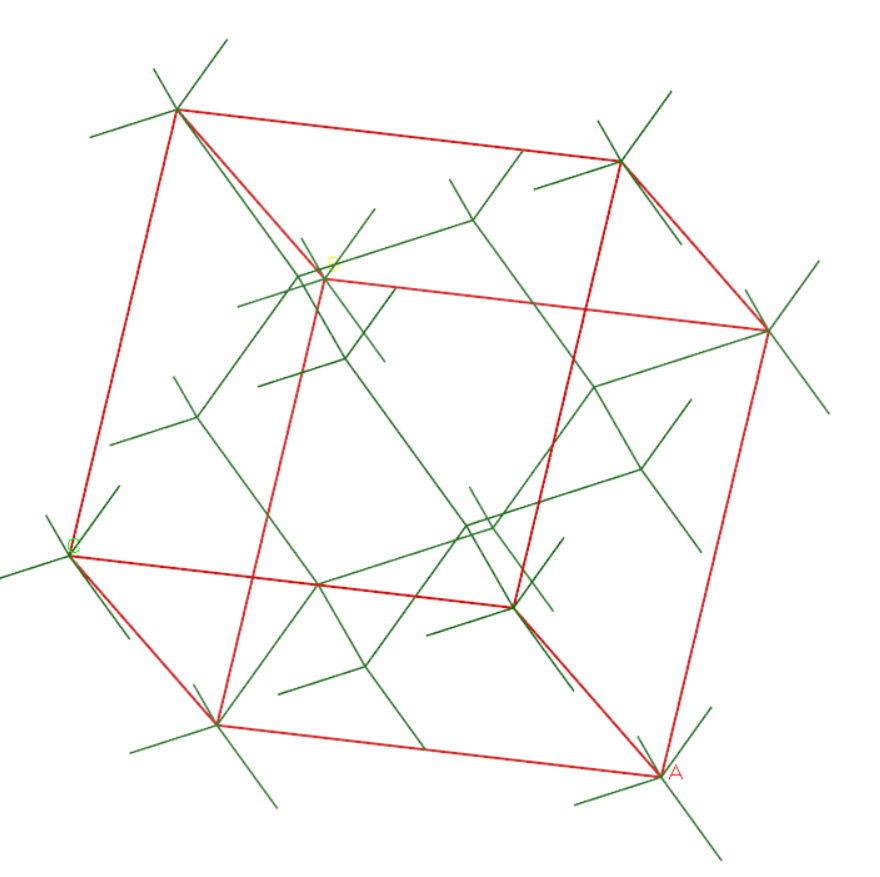
\includegraphics[width=\linewidth]{screenshots/unit-cell.png}
    \end{subfigure}
    \begin{subfigure}[c]{0.4\linewidth}
        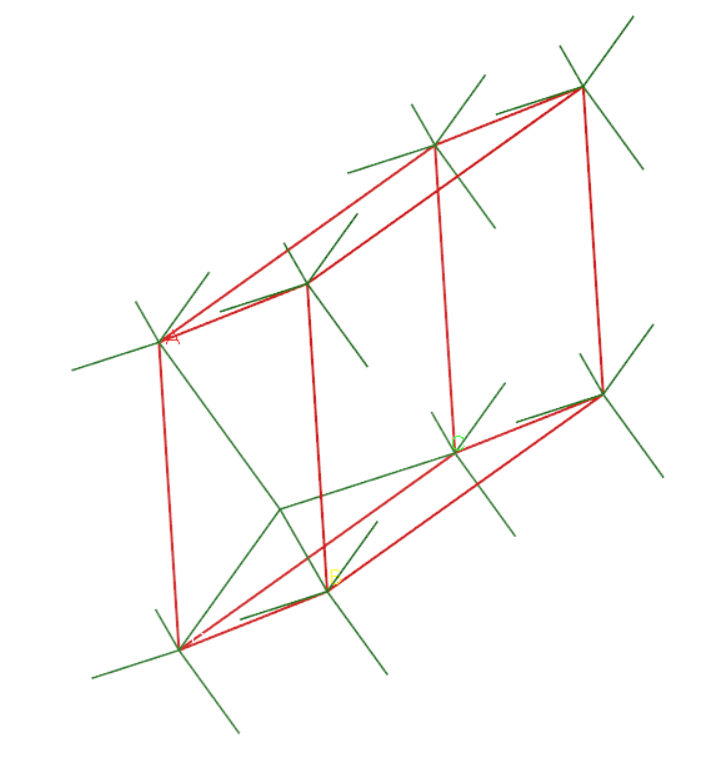
\includegraphics[width=\linewidth]{screenshots/primitve-cell.png}
    \end{subfigure}
    \caption{Material Studio 中晶体的晶胞与原胞}\label{fig:ms-cells}
\end{figure}

\subsection{布里渊区与 K 路径}

我们考虑金刚石型晶体——或更一般的,面心立方晶体的布里渊区的结构。

\begin{proposition}
    面心立方晶体的(第一)布里渊区是倒空间中的截角八面体(truncated octahedron),即从正八面体的角上截去六个相同的四棱锥形成的多面体,如图~\ref{fig:truncated-octahedron}所示。
\end{proposition}

\begin{figure}[ht!]
    \centering
    \begin{asy}
    include "./truncated-octahedron.asy";
    \end{asy}
    \caption{倒空间中的截角八面体,从四根轴中任取三根即可组成倒空间的基底。}
    \label{fig:truncated-octahedron}
\end{figure}

\begin{proof}
    不妨设面心立方晶胞的边长为$\frac{2}{\pi}$,考虑正空间中的原胞产生的格点的基底
    \begin{equation}
        a_1 = (\frac{1}{\pi}, \frac{1}{\pi}, 0), \; a_2 = (\frac{1}{\pi}, 0, \frac{1}{\pi}), \; a_3 = (0, \frac{1}{\pi}, \frac{1}{\pi}).
    \end{equation}
    对应的倒空间基底自然为
    \begin{equation}
        b_1 =  (1, 1, -1), b_2 = (1, -1, 1), b_3 = (- 1, 1, 1).
    \end{equation}
    这三个基底向量和$(-1,-1,-1)$将倒空间分为对称的四个部分。
    由于原胞的基底不正交,倒空间的基底也不正交,其立体夹角为
    \begin{equation}
        \phi = \arccos \frac{b_1 \cdot b_2}{\Vert b_1 \Vert \cdot \Vert b_2 \Vert} \approx \ang{109.47}.
    \end{equation}
    我们现在仅考虑一个卦限中的情况,其他情况可容易地根据对称性推出,考虑与原点紧邻的七个格点,首先在倒空间基底中写出其坐标:
    \begin{equation}
        \begin{aligned}
            A(1, 0, 0), B(0, 1, 0), C(0, 0, 1), D(1, 1, 1) \\
            E(1, 1, 0), F(1, 0, 1), G(0, 1, 1), 
        \end{aligned}
    \end{equation}
    然后回到笛卡尔坐标系中,首先注意$A, B, C, D$:
    \begin{equation}
        A' (1, 1, -1), B' (1, -1, 1), C'(-1, 1, 1), D'(1, 1, 1),
    \end{equation}
    从原点到这四个点的连线的垂直平分面截成了正八面体的一部分,而剩下三个点的垂直平分面则从这个正八面体中截除了全等的三个四棱锥。
\end{proof}

为在 Material Studio 中给出第一布里渊区的形状与自动计算的 K 路径,首先选择构建(Build)、对称性(Symmetry)、原胞(Primitive Cell)来展示晶胞的原胞视图。
然后选择工具(Tools)、布里渊区路径(Brillouin Zone Path)即可生成K路径。
图~\ref{ref:ms-brillouin-zone}展示了上述操作的结果。

\begin{figure}[ht!]
    \centering
    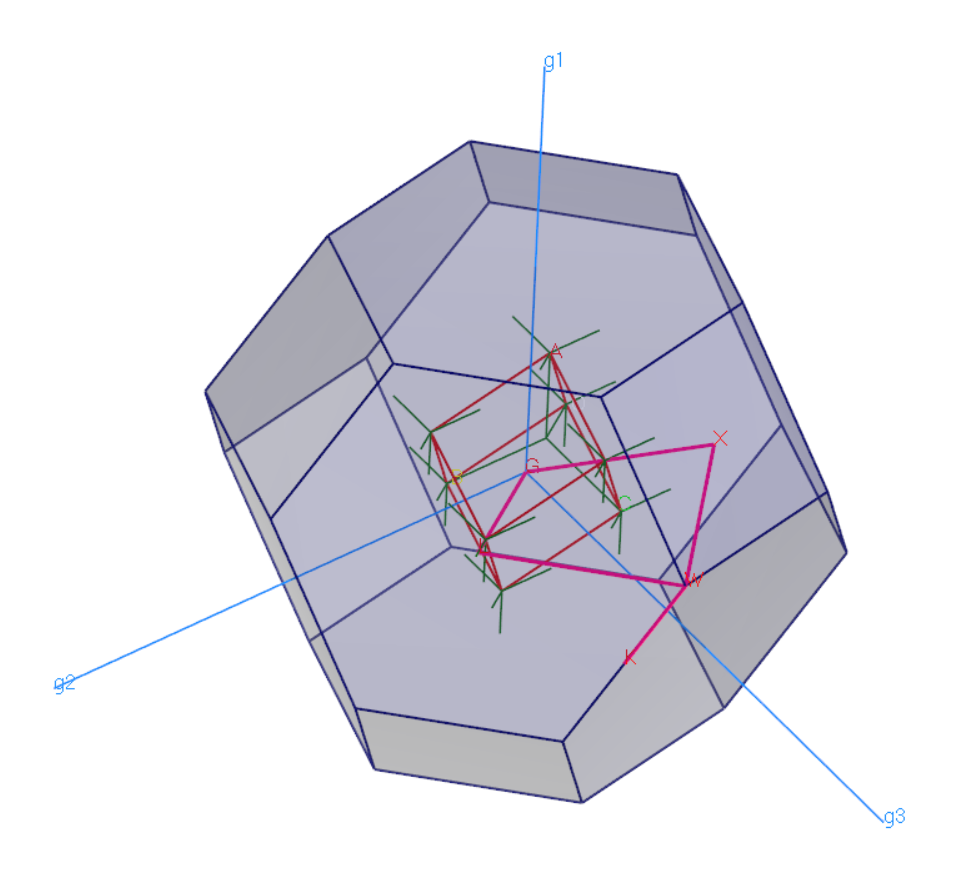
\includegraphics[width=0.8\linewidth]{screenshots/reciprocal.png}
    \caption{Material Studio 中的布里渊区与路径。}
    \label{ref:ms-brillouin-zone}
\end{figure}

\subsection{计算能带}

最后,我们以能带为例展示在 Material Studio 中计算物质性质的步骤。
首先,选择计算使用的软件包,此处我们选择 CASTEP 包。

在保持最初的原子结构文件打开的情况下,从菜单栏中选择 CASTEP 计算(CASTEP Tools \verb|->| Calculation)。
根据 CASTEP 包的说明,我们首先需要计算能量,然后才能给出晶体的属性。
在“任务”(Task)下拉菜单中选择“能量”(Energy),计算品质选择“精细”(Fine),取消勾选“金属”(Metallic)选项,其他设置保持默认,然后在“属性”(Properties)选项卡中勾选需要的“属性”,单击运行(Run)开始计算。
此处我们选择的属性有“能带结构”(Band structure)、“态密度”(Density of states)和“声子”(Phonons),为计算声子,必须选择保范数的赝势。
在作业(Jobs)窗口中观察,等待任务完成。

任务完成以后,项目中会生成多种文件,包括记录晶体结构的 \verb|*.xsd| 文件和计算参数的 \verb|*.param| 文件、输出的 \verb|status.txt| 日志文件、计算中使用的参考文献生成的 \verb|*.bib| 文件以及计算的结果。

首先考虑 \verb|status.txt| 文件,该文件包括以下内容:
\begin{enumerate}
    \item 标头,包括进行计算的时间、计算机名和软件包信息等;
    \item 结果概况,包括原子信息、使用的赝势、收敛迭代数(\texttt{Converged in 54 iterations ...})和本征值等;
    \item 配置信息,此处基本是 Material Studio 默认的配置;
    \item 计算参数,包括原胞的各种参数、原子的位置和对称性等;
    \item 尾部,包括计算使用的时间。
\end{enumerate}

为分析能带结构,需选择“分析”(Analysis)选项并选择“能带结构”(Band structure),勾选“能带密度”(DOS)并确认即可画图,图~\ref{fig:si-band-structure-castep}展示了CASTEP 计算的能带的结构。

\begin{figure}[ht!]
    \centering
    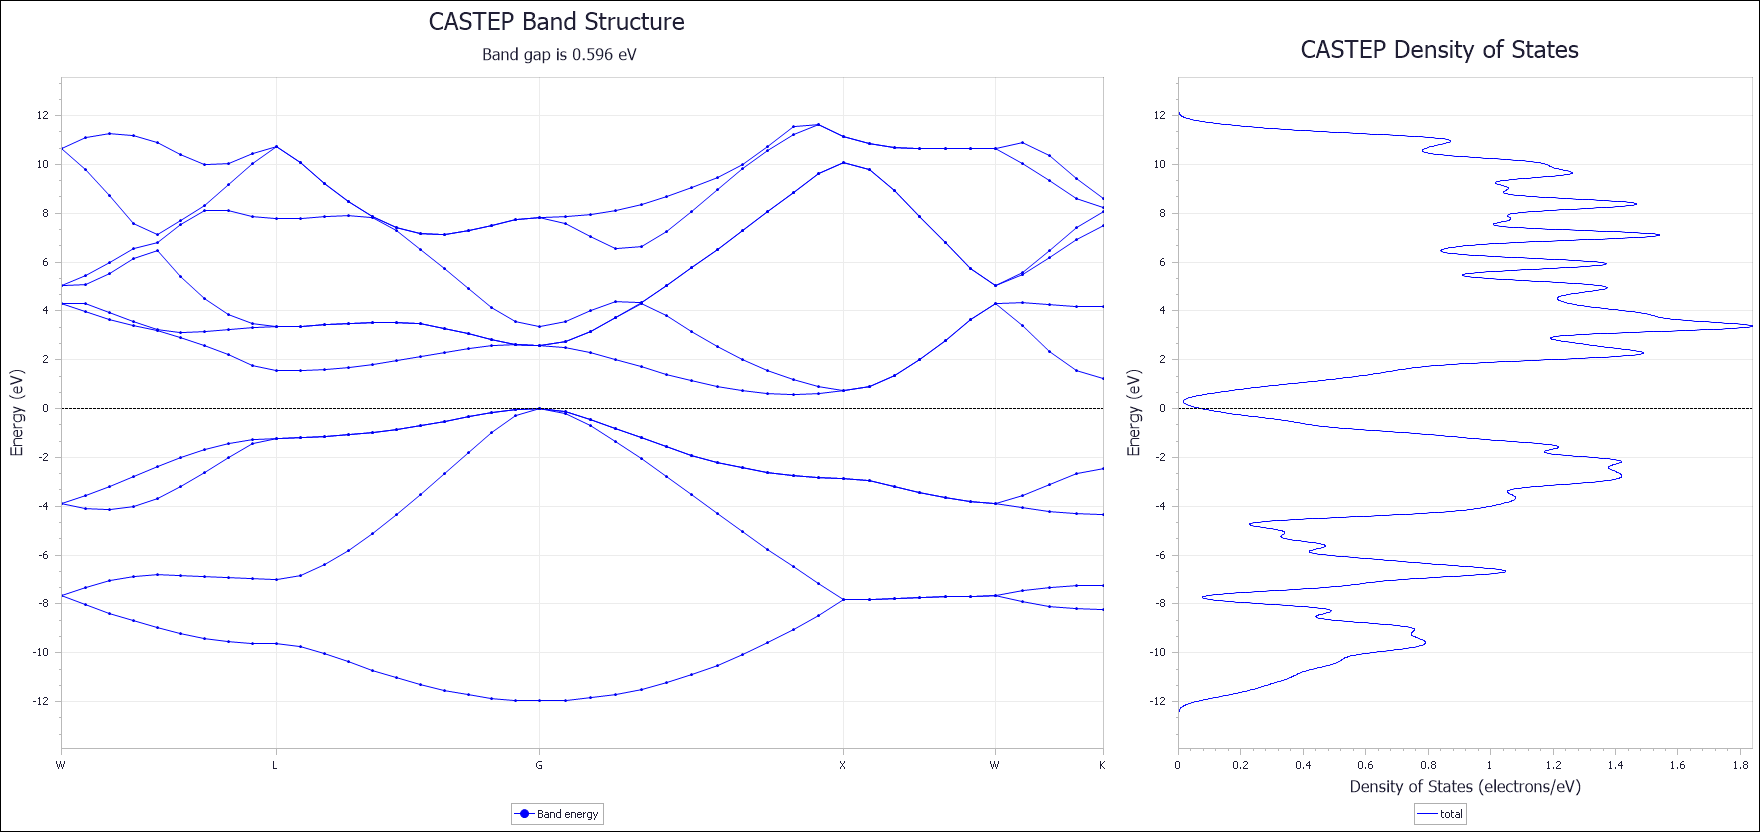
\includegraphics[width=0.9\linewidth]{results/si-band-structure-castep.png}
    \caption{CASTEP 计算的能带结构。}
    \label{fig:si-band-structure-castep}
\end{figure}

\begin{figure}[ht!]
    \centering
    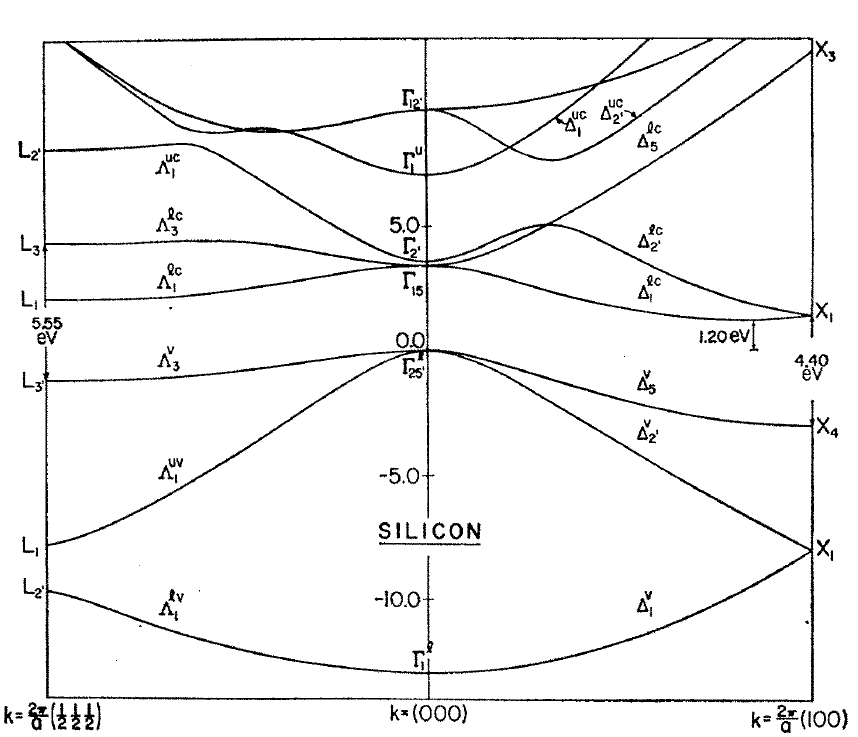
\includegraphics[width=0.6\linewidth]{results/si-band-structure-reference.png}
    \caption{Si 的能带结构,来自 \cite{cardona_energy_band_1966}。}
    \label{fig:si-band-structure-reference}
\end{figure}

与图~\ref{fig:si-band-structure-reference}比较,可见 CASTEP 计算出的能带结构与前人计算的大致相符\cite{phillips_band_1962,cardona_energy_band_1966},但是带隙显著低于测量值($\qty{1.20}{\electronvolt}$左右)。

带隙显著低于测量值是 CASTEP 等使用的密度泛函理论(Density-Functional Theory,DFT)计算的一大特点。
该理论通过计算单一电子加入基态绝缘体系统(即满带)产生的能量变化来求解带隙。
根据定义,带隙的能量为
\begin{equation}
    E_g = (E_{n+1} - E_n) - (E_n - E_{n-1}),
\end{equation}
因此,只要能够准确地计算基态电子的能量,就可以求出带隙的能量。
但是由于电子的交换-相关势能(exchange-correlation potential)在该情况下存在不连续的断点,因此DFT理论无法给出对新增电子的基态能量的准确估计,从而无法给出准确的带隙,这一问题称为“带隙问题”(Band gap problem)\cite{borlido_exchange-correlation_2020,sham_density-functional_1983}。

计算出的声子数据可用于预测材料的热力学数据,如图~\ref{fig:si-thermodynamics}所示。
\begin{figure}
    \centering
    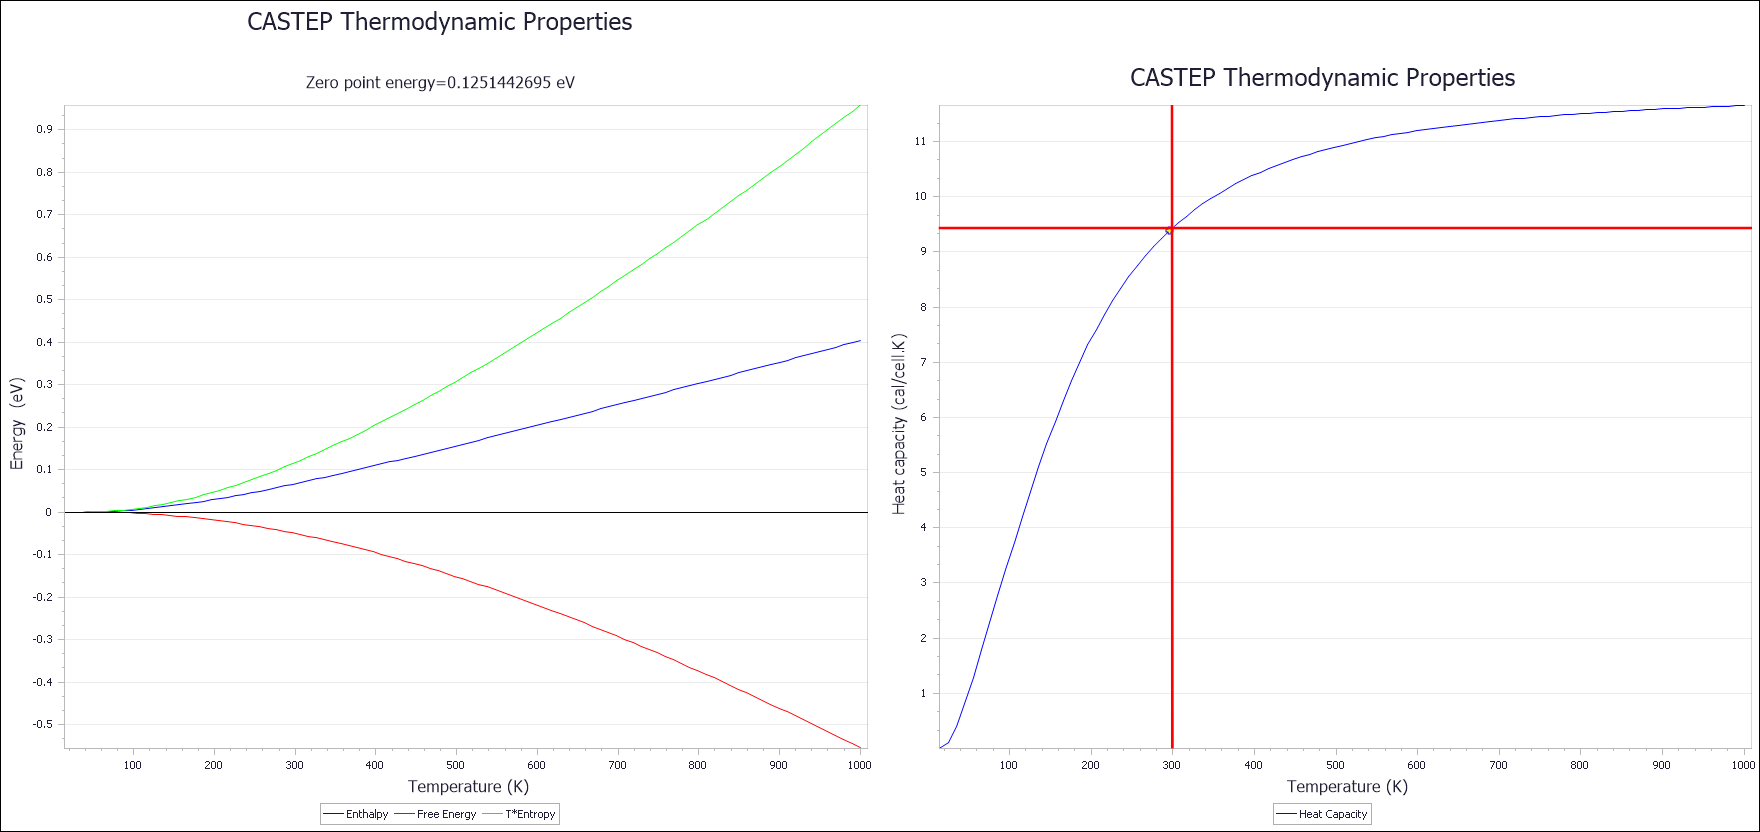
\includegraphics[width=0.8\linewidth]{results/si-thermodynamics.png}
    \caption{CASTEP 预测的热力学数据。}
    \label{fig:si-thermodynamics}
\end{figure}
从图中可读出$\qty{300}{\kelvin}$时比热约为
\begin{equation}
    \qty{9.4}{\calUnit\per\cell\per\kelvin} = 9.4 \times \frac{4.184}{2} \; \unit{\joule\per\mole\per\kelvin} = \qty{19.66}{\joule\per\mole\per\kelvin},
\end{equation}
与实验数据($\qty{20.05}{\joule\per\mole\per\kelvin} \; @ \; \qty{300}{\kelvin}$)较为符合。
